\documentclass[a4paper,12pt]{article}

% 导言区
\usepackage{titlesec}
\usepackage{lipsum} % 示例用,可以删除
\usepackage{geometry}
\usepackage{setspace}
\usepackage{amsmath} % 用于数学公式
\usepackage{graphicx} % 用于插入图片
\usepackage{float}
\usepackage{ctex} % 导入 ctex 包以支持中文
\usepackage{xeCJK}
\usepackage{titlesec} % 导入 titlesec 包以定制标题样式
\usepackage{fontspec} % 用于设置中文字体
\usepackage{array}


% 目录设置
\usepackage[nottoc,notlot,notlof]{tocbibind}
\usepackage{enumitem}

% 页面设置
\geometry{margin=1in}

% 标题设置
\titleformat{\section}{\normalfont\Large\bfseries}{\thesection}{1em}{}
\titleformat{\subsection}{\normalfont\large\bfseries}{\thesubsection}{1em}{}
\titleformat{\subsubsection}{\normalfont\normalsize\bfseries}{\thesubsubsection}{1em}{}

% 行间距设置
\onehalfspacing

% 文档信息
\title{启发式评估报告}
\author{人机不寄小分队}
\date{\today}

\begin{document}

\maketitle

% 添加目录
\tableofcontents

\section{团队成员}
211250124 程智镝

211250122 刘辉

211250159 陈凌

211250158 李忠信

\section{文档概况}
\subsection{文档负责人员}
\begin{tabular}{|c|c|c|c|}
    \hline
    姓名   & 学号     & 负责任务   \\
    \hline
    程智镝 & 211250124& 组长,分配任务    \\
    陈凌 & 211250159& 分析可用性问题    \\
    刘辉 & 211250122& 分析可用性问题    \\
    李忠信 & 211250158& 分析可用性问题   \\
    \hline
\end{tabular}

\section{评估对象}
20足迹相册地图    
评估对象组 :刘永全,李博轩,张涵景,马培森

网址:\verb|https://git.nju.edu.cn/micer/HCI_frontend.git|

此项目描述了 基于地理位置的相册应用,用户可以在应用中上传自己拍摄的照片,并添加地理位置信息和描述。这些照片会在地图上标记出来,用户可以通过地图浏览自己和其他用户上传的照片,以及搜索特定地点或附近地点的照片。该应用旨在让用户通过地图的方式记录和分享自己的足迹,发现世界各地的美景和有趣的地点。同时,应用也会考虑用户体验和数据安全,保证用户可以方便地上传和浏览照片,并保护用户的隐私信息。

功能:
\begin{enumerate}
    \item 用户上传照片:用户可以上传自己拍摄的照片到应用中。
    \item 添加地理位置信息和描述:用户可以为上传的照片添加地理位置信息和描述,以便在地图上进行标记和展示。
    \item 查看地图上的照片标记:用户可以在地图上浏览自己和其他用户上传的照片标记。
    \item 搜索特定地点的照片:用户可以通过搜索功能查找特定地点或者附近地点上传的照片。
    \item 浏览他人上传的照片:用户可以浏览其他用户上传的照片,并了解他们在不同地点的足迹和体验。
\end{enumerate}

\section{评估方法}
\subsection{评估流程}
\begin{enumerate}
    \item 准备:确定可用性准则与评估记录策略。
    \item 评估:尝试并建立对系统概况的感知
    \item 结果分析:回顾每个评估者记录的每个问题并分析。
    \item 报告汇总:对严重性进行划分。
\end{enumerate}

\subsection{启发式评估标准}
我们启发式评估采用的准则为 Nielsen 的 10 条启发式评估准则:
\begin{enumerate}
    \item Visibility of system status
    \item Match between system and the real world
    \item User control and freedom
    \item Consistency and standards
    \item Error prevention
    \item Recognition rather than recall
    \item Flexibility and efficiency of use
    \item Aesthetic and minimalist design
    \item Help users recognize, diagnose, and recover from errors
    \item Help and documentation
\end{enumerate}

\subsection{严重性等级的标准}
\begin{tabular}{|c|p{10cm}|}
    \hline
    等级 & 定义和描述 \\
    \hline
    0 & 非关键问题或关于产品的一般性问题。有些细微的不一致会引起犹豫或美学上的小问题。 例如:打字错误(如果是在关键的地方,比如菜单或闪屏上,这可能是一个更高的优先级);菜单项不使用推荐的字符。 \\
    \hline
    1 & 非关键的、有限的问题(没有数据丢失或系统故障)。它不妨碍操作,可以暂时避免。这个问题会给用户带来一定程度的困惑或烦恼。 例如:一个普通的菜单项或工具栏按钮不能做通常期望的事情;明显的性能效率低下。 \\
    \hline
    2 & 损害一种或多种产品功能的运行或持续运行,且无法轻易规避或避免的严重状况。该软件不能防止用户犯严重的错误。可用性问题是频繁的、持久的,并且影响许多用户。 例如:缺少关键操作的反馈;没有键盘访问方法的功能。 \\
    \hline
    3 & 一种导致客户系统故障或导致客户数据丢失或销毁的紧急情况。这些问题没有解决办法。许多客户需要的关键特性不在系统中。 例如:可用性问题很可能导致一个错误,这会让客户浪费大量的时间或金钱;可用性 \\
    \hline
\end{tabular}

\subsection{修复等级的标准}
\begin{tabular}{|c|p{10cm}|}
    \hline
    等级 & 定义和描述 \\
    \hline
    0 & 非常容易修复,由一个项目组成员能够完成。 \\
    \hline
    1 & 容易修复,涉及到特定界面元素,有明确解决方案。 \\
    \hline
    2 & 修复有些困难,涉及界面的很多方面,需要整个项目组成员来完成或者解决方案尚不明确。 \\
    \hline
    3 & 难以修复,在下一版本发布之前解决有一定难度,尚未获得明确的解决方案或是解决方案仍存有争议。 \\
    \hline
    \end{tabular}
    
\section{评估环境}
所有评估都在电脑网站浏览器上面运行与测试,使用的网络为南京大学校园网。
使用的是 chrome 浏览器
\section{评估结果}
\subsection{可用性问题}
\begin{tabular}{|m{3cm}<{\centering}|p{10cm}|}
	\hline
	编号 & 1 \\
	\hline
	界面位置和功能 & 首页的中国地图的地区图示 \\
	\hline
	可用性问题 & 不同地区的名字重叠在一起,难以看清和辨认 \\
	\hline
	严重性等级 & 2 \\
	\hline
	修复等级 & 1 \\
	\hline
	违反规则 & 规则6、规则8 \\
	\hline
	改进建议 & 对不同地区的名字的排布进行更加合理有序的排版,或者将整幅地图放大一些,使得地区名字更清晰可见 \\
	\hline
	界面截图 & 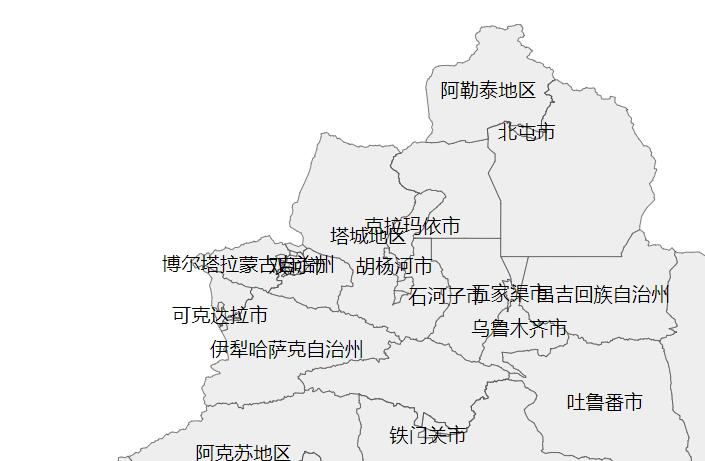
\includegraphics[width=6cm, height=4cm]{q1.jpg} \\
	\hline
\end{tabular}

\vspace{2em}

\begin{tabular}{|c|p{10cm}|}
	\hline
	编号 & 2 \\
	\hline
	界面位置和功能 & 首页 \\
	\hline
	可用性问题 & 在滑动鼠标滚轮时会缩放页面,但是界面上的元素会出现移位、错位问题 \\
	\hline
	严重性等级 & 2 \\
	\hline
	修复等级 & 2 \\
	\hline
	违反规则 & 规则3 \\
	\hline
	改进建议 & 删除或者改进界面的缩放操作,保持界面元素布局的一致性 \\
	\hline
	界面截图 & 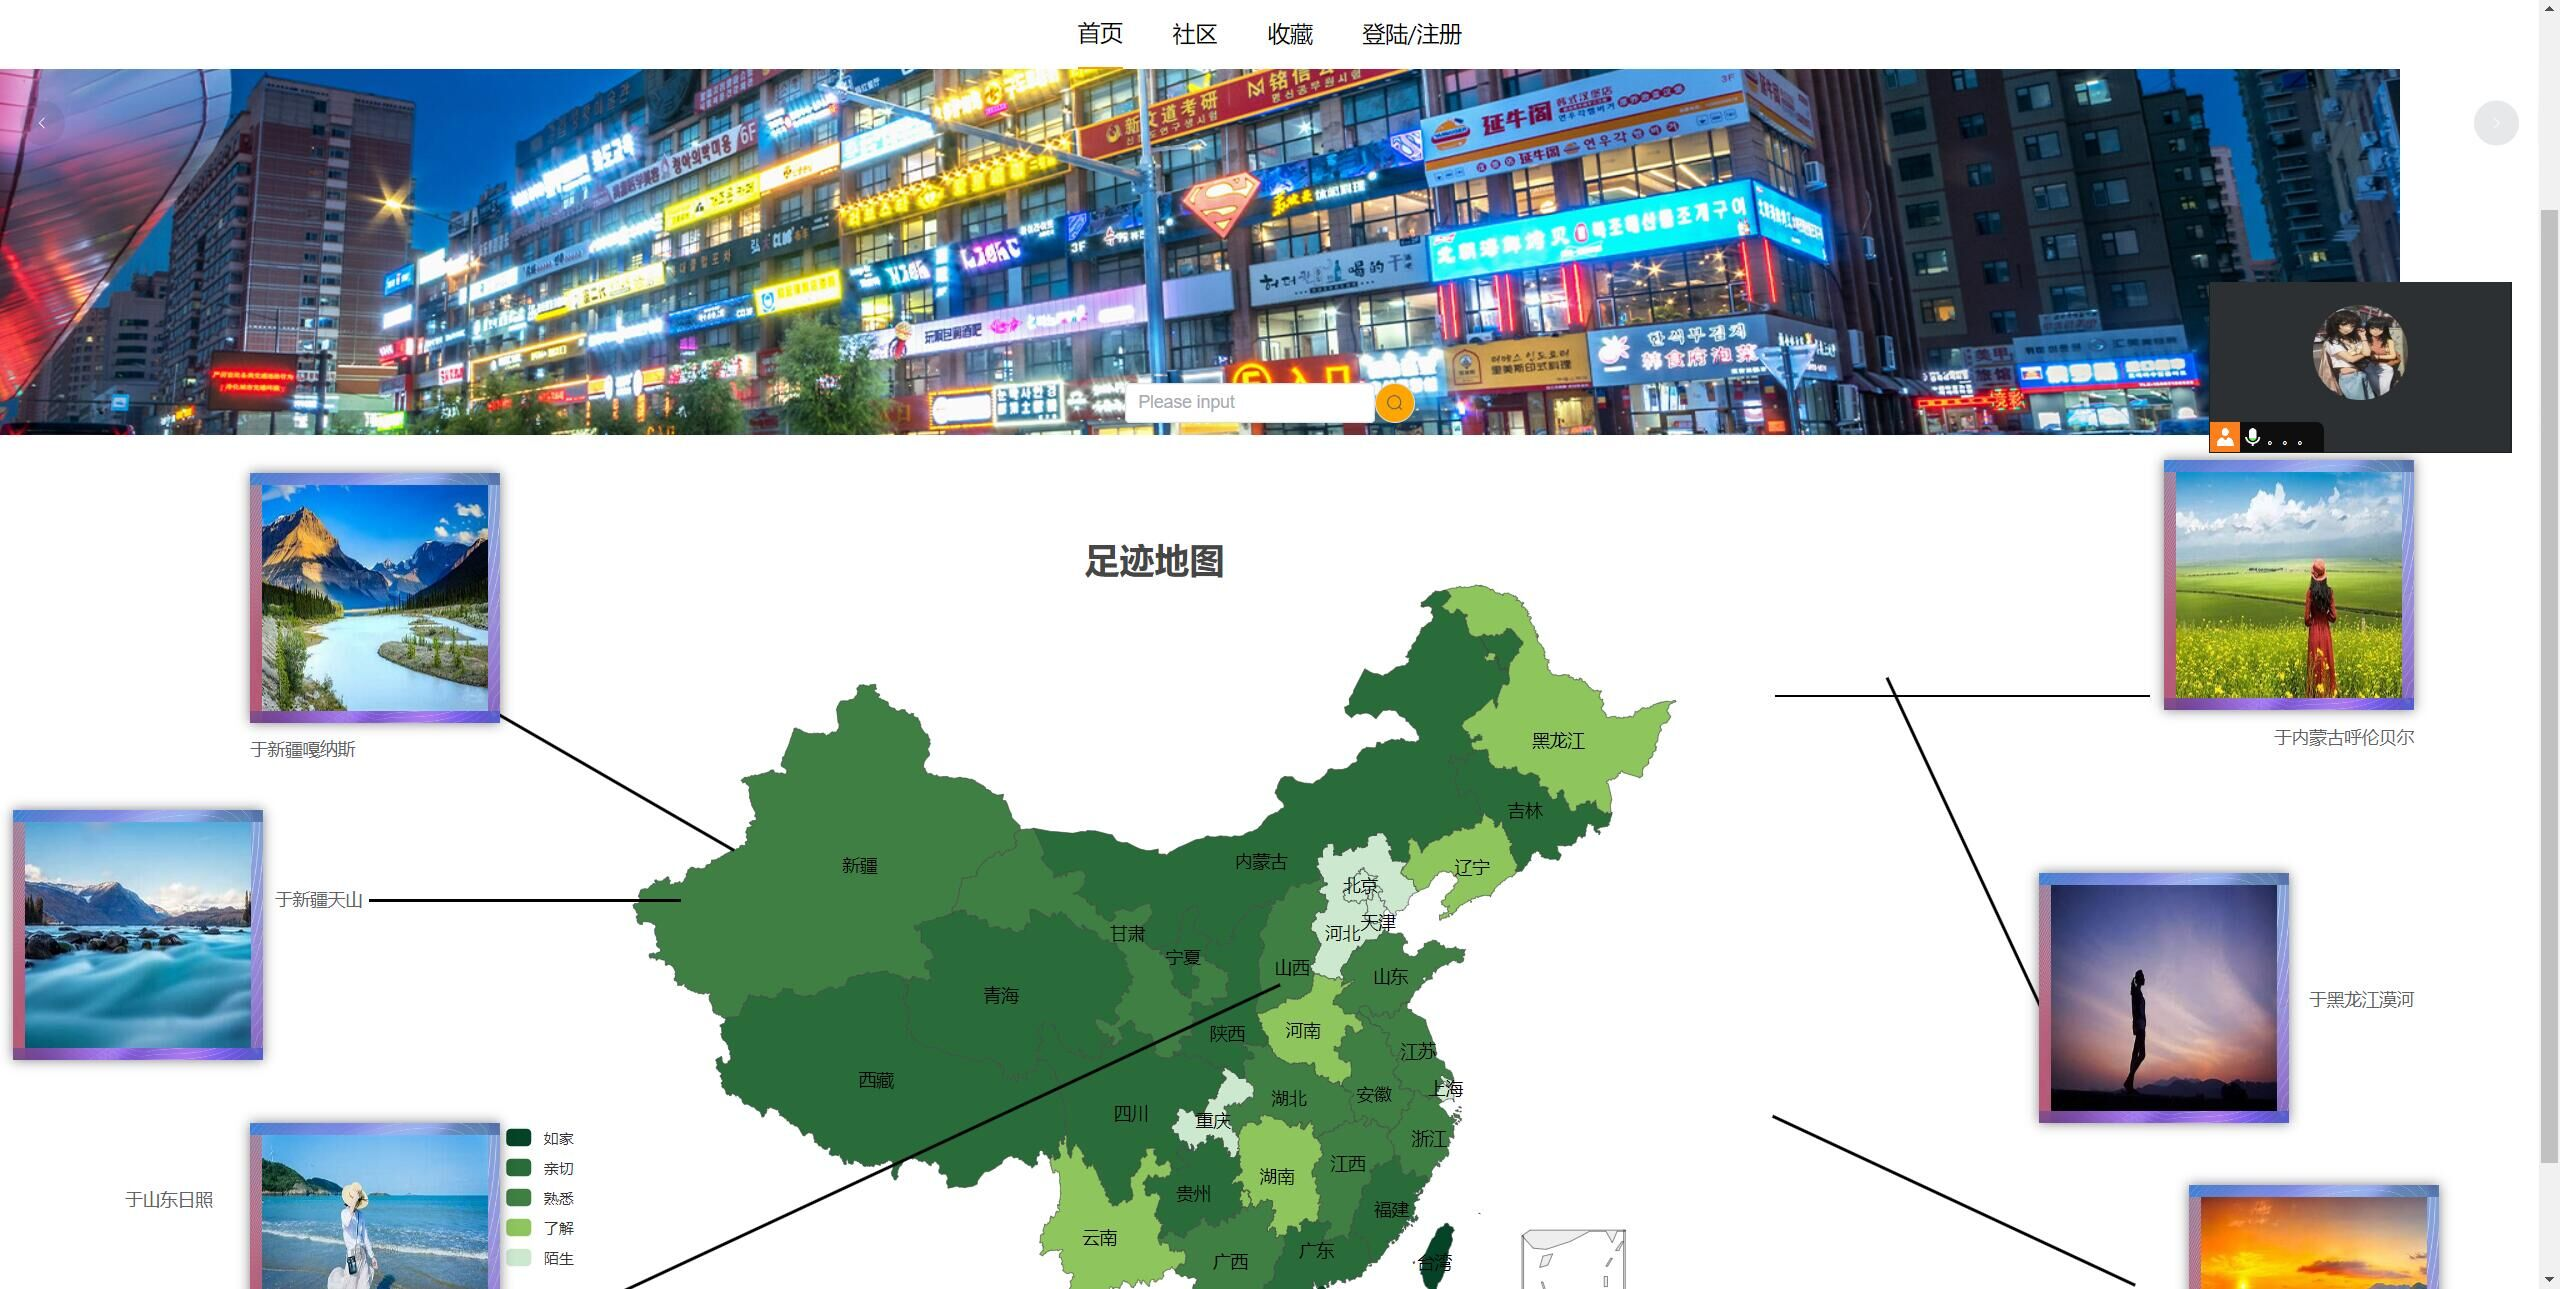
\includegraphics[width=8cm, height=4cm]{q2.jpg} \\
	\hline
\end{tabular}

\vspace{2em}

\begin{tabular}{|m{3cm}<{\centering}|p{10cm}|}
	\hline
	编号 & 3 \\
	\hline
	界面位置和功能 & 地图详情页 \\
	\hline
	可用性问题 & 返回按钮位置不显眼,且不美观 \\
	\hline
	严重性等级 & 0 \\
	\hline
	修复等级 & 1 \\
	\hline
	违反规则 & 规则8 \\
	\hline
	改进建议 & 对返回按键进行更加合理有序的排版,使其更容易被用户发现并使用,同时提升界面的美观性 \\
	\hline
	界面截图 & 
\includegraphics[width=3cm, height=2cm]{q3.jpg} \\
	\hline
\end{tabular}

\vspace{2em}

\begin{tabular}{|m{3cm}<{\centering}|p{10cm}|}
	\hline
	编号 & 4 \\
	\hline
	界面位置和功能 & 登录注册界面 \\
	\hline
	可用性问题 & 登录时有背景,而切换到注册背景消失,且登录框与背景的结合影响观感,不容易看清 \\
	\hline
	严重性等级 & 0 \\
	\hline
	修复等级 & 1 \\
	\hline
	违反规则 & 规则8 \\
	\hline
	改进建议 & 修改注册页面使背景能正常显示,修改背景图片使其能覆盖全部页面,或修改登录框透明度 \\
	\hline
	界面截图 & 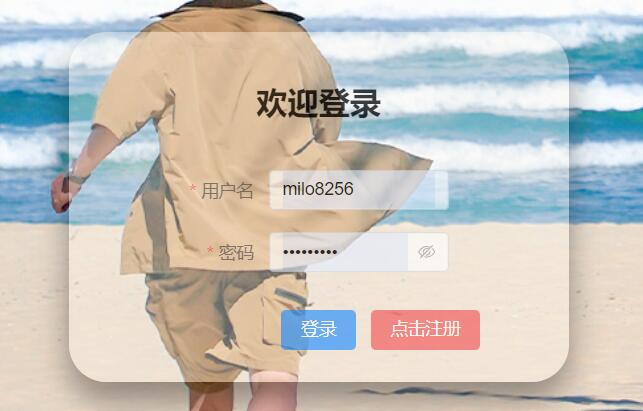
\includegraphics[width=6cm, height=4cm]{q4.jpg} \\
	\hline
\end{tabular}

\vspace{2em}

\begin{tabular}{|c|p{10cm}|}
	\hline
	编号 & 5 \\
	\hline
	界面位置和功能 & 登录/注册时的操作提示 \\
	\hline
	可用性问题 & 提示框出现在屏幕的中心线上,且不包含操作成功或失败的相关信息 \\
	\hline
	严重性等级 & 2 \\
	\hline
	修复等级 & 1 \\
	\hline
	违反规则 & 规则1、规则9 \\
	\hline
	改进建议 & 将提示框的位置放到界面的右上角,并且给出相关操作结果的具体信息 \\
	\hline
	界面截图 & 
\includegraphics[width=9cm, height=2cm]{q5.jpg} \\
	\hline
\end{tabular}

\vspace{2em}

\begin{tabular}{|c|p{10cm}|}
	\hline
	编号 & 6 \\
	\hline
	界面位置和功能 & 首页搜索地点的输入框 \\
	\hline
	可用性问题 & 由于在首页上输入框的大小比较小而且跟某些背景图片的颜色很相似,用户可能找不到输入框的位置;并且输入框中没有有效的输入提示来告诉用户应该输入什么 \\
	\hline
	严重性等级 & 1 \\
	\hline
	修复等级 & 0 \\
	\hline
	违反规则 & 规则8、规则10 \\
	\hline
	改进建议 & 将输入框的放在更加显眼的位置如白色背景处,并且给出输入的操作提示和例子 \\
	\hline
	界面截图 & 
\includegraphics[width=9cm, height=2cm]{q6.jpg} \\
	\hline
\end{tabular}

\vspace{2em}

\begin{tabular}{|c|p{10cm}|}
	\hline
	编号 & 7 \\
	\hline
	界面位置和功能 & 首页搜索地点的输入框的操作提示 \\
	\hline
	可用性问题 & 首页上输入框的操作结果提示与登录/注册时的操作结果提示的内容风格不一致\\
	\hline
	严重性等级 & 0 \\
	\hline
	修复等级 & 0 \\
	\hline
	违反规则 & 规则4 \\
	\hline
	改进建议 & 将首页上输入框的操作结果提示与登录/注册时的操作结果提示的内容风格统一,都改为首页输入框的操作结果提示的风格 \\
	\hline
	界面截图 & 
\includegraphics[width=9cm, height=2cm]{q7.jpg} \\
	\hline
\end{tabular}

\end{document}
